\begin{figure}[ht]
	\centering
	\footnotesize

	\psfrag{fo}[c][c] {$\textbf{\large First order}$}
	\psfrag{ho}[c][c] {$\textbf{\large Higher order}$}

	\psfrag{li}[c][c] {$\textbf{\large Linear}$}
	\psfrag{noli}[c][c] {$\textbf{\large Nonlinear}$}

	\psfrag{mo}[l][l] {$\bullet \text{ \large \textit{monotone}}$}
	\psfrag{l1c}[l][l] {$\bullet \text{ \large $L_1$-\textit{contracting}}$}
	\psfrag{tvd}[l][l] {$\bullet \text{ \large TVD}$}
	\psfrag{mop}[l][l] {$\bullet \text{ \large \textit{monotonicity-preserving}}$}

	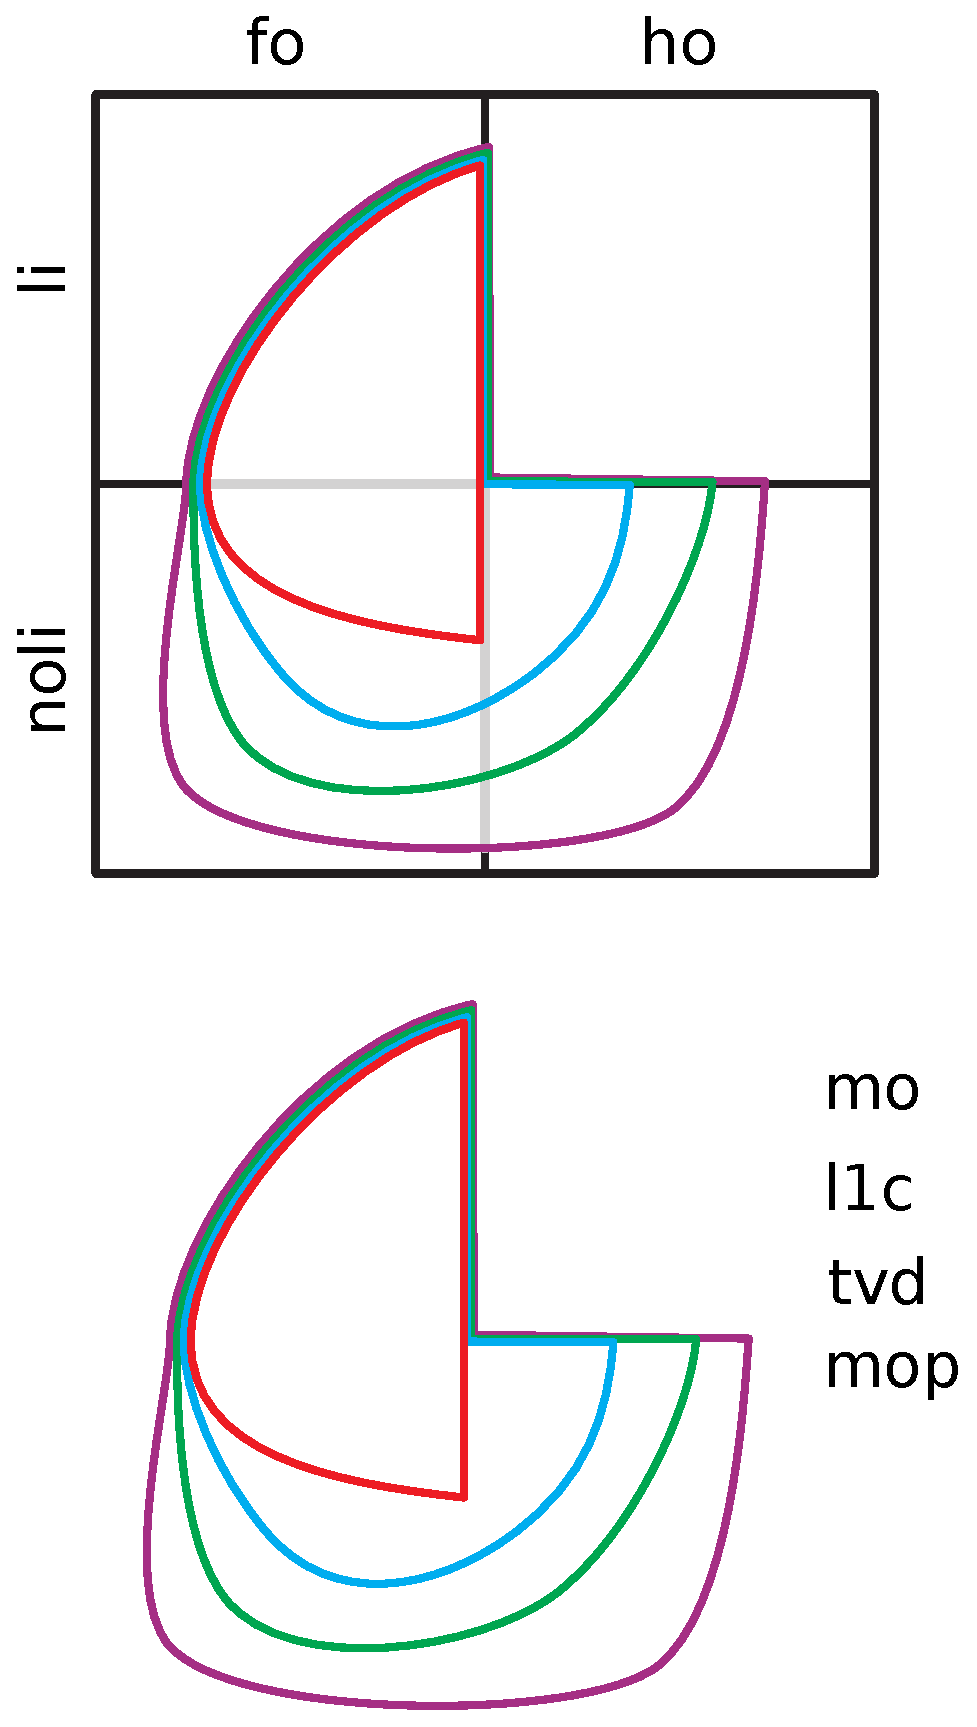
\includegraphics[width=0.62\textwidth]{structureFVM.eps}
	\caption{Structure of Finite Volume Method [Lecture note page 115].}
	\label{\LABEL}
\end{figure}
